\documentclass[a4paper, 12pt]{article}

%% Created with wxMaxima 23.05.1

\setlength{\parskip}{\medskipamount}
\setlength{\parindent}{0pt}
\usepackage{iftex}
\ifPDFTeX
  % PDFLaTeX or LaTeX 
  \usepackage[utf8]{inputenc}
  \usepackage[T1]{fontenc}
  \DeclareUnicodeCharacter{00B5}{\ensuremath{\mu}}
\else
  %  XeLaTeX or LuaLaTeX
  \usepackage{fontspec}
\fi
\usepackage[russian]{babel}.
\usepackage{graphicx}
\usepackage{color}
\usepackage[top=2.5cm, bottom=2.5cm, left=2cm, right=2cm]{geometry}
\usepackage{amsmath}
\usepackage{grffile}
\usepackage{ifthen}
\newsavebox{\picturebox}
\newlength{\pictureboxwidth}
\newlength{\pictureboxheight}
\newcommand{\includeimage}[1]{
    \savebox{\picturebox}{\includegraphics{#1}}
    \settoheight{\pictureboxheight}{\usebox{\picturebox}}
    \settowidth{\pictureboxwidth}{\usebox{\picturebox}}
    \ifthenelse{\lengthtest{\pictureboxwidth > .95\linewidth}}
    {
        \includegraphics[width=.95\linewidth,height=.80\textheight,keepaspectratio]{#1}
    }
    {
        \ifthenelse{\lengthtest{\pictureboxheight>.80\textheight}}
        {
            \includegraphics[width=.95\linewidth,height=.80\textheight,keepaspectratio]{#1}
            
        }
        {
            \includegraphics{#1}
        }
    }
}
\newlength{\thislabelwidth}
\DeclareMathOperator{\abs}{abs}

\definecolor{labelcolor}{RGB}{100,0,0}



\begin{document}
\title{ВВОДНОЕ ЗАНЯТИЕ. ОСНОВЫ РАБОТЫ В MAXIMA}
\author{Дарья Рузанова}
{\let\newpage\relax\maketitle}
\tableofcontents
\section{Исследование функции}
% \newpage

\noindent
%%%%%%%%
%% INPUT:
\begin{minipage}[t]{4.000000em}\color{red}\bfseries
(\% i4)	
\end{minipage}
\begin{minipage}[t]{\textwidth}\color{blue}
f(x,\ y)\ :=\ 2*(x\^\ 4)-24*(x\^\ 3)\ +\ 107*(x\^\ 2)\ -210*(x)\ +\ y\^\ 4\ -\ 8*(y\^\ 3)\ +\ 22*(y\^\ 2)\ -24*y\ +\ 161;
\end{minipage}
%%%% OUTPUT:
\[\displaystyle \tag{\% o4} 
\operatorname{f}\left( x\operatorname{,}y\right) \operatorname{:=}2 {{x}^{4}}\operatorname{-}24 {{x}^{3}}\operatorname{+}107 {{x}^{2}}\operatorname{+}\operatorname{-}210 x\operatorname{+}{{y}^{4}}\operatorname{+}\operatorname{-}8 {{y}^{3}}\operatorname{+
}22 {{y}^{2}}\operatorname{+}\operatorname{-}24 y\operatorname{+}161\mbox{}
\]
%%%%%%%%%%%%%%%%


\noindent
%%%%%%%%
%% INPUT:

Находим частные производные нашей функции

\begin{minipage}[t]{4.000000em}\color{red}\bfseries
(\% i15)	
\end{minipage}
\begin{minipage}[t]{\textwidth}\color{blue}
dif\_x:\ diff(f(x,\ y),x,1);
\end{minipage}
%%%% OUTPUT:
\[\displaystyle \tag{dif\_ x} 
8 {{x}^{3}}\operatorname{-}72 {{x}^{2}}\operatorname{+}214 x\operatorname{-}210\mbox{}
\]
%%%%%%%%%%%%%%%%


\noindent
%%%%%%%%
%% INPUT:
\begin{minipage}[t]{4.000000em}\color{red}\bfseries
(\% i16)	
\end{minipage}
\begin{minipage}[t]{\textwidth}\color{blue}
dif\_y:\ diff(f(x,\ y),y,1);
\end{minipage}
%%%% OUTPUT:
\[\displaystyle \tag{dif\_ y} 
4 {{y}^{3}}\operatorname{-}24 {{y}^{2}}\operatorname{+}44 y\operatorname{-}24\mbox{}
\]
%%%%%%%%%%%%%%%%


\noindent
%%%%%%%%
%% INPUT:
Решим систему уравнений, чтобы найти критические точки.

\begin{minipage}[t]{4.000000em}\color{red}\bfseries
(\% i29)	
\end{minipage}

\begin{minipage}[t]{\textwidth}\color{blue}
candidates:\ solve([dif\_x\ =\ 0,\ dif\_y\ =\ 0],\ [x,\ y]);
\end{minipage}
%%%% OUTPUT:
\[\displaystyle \tag{candidates} 
\operatorname{[}\left[ x\operatorname{=}\frac{5}{2}\operatorname{,}y\operatorname{=}1\right] \operatorname{,}\left[ x\operatorname{=}\frac{7}{2}\operatorname{,}y\operatorname{=}1\right] \operatorname{,}\left[ x\operatorname{=}3\operatorname{,}y\operatorname{=}1\right] \operatorname{,
}\left[ x\operatorname{=}\frac{5}{2}\operatorname{,}y\operatorname{=}2\right] \operatorname{,}\]
\[\left[ x\operatorname{=}\frac{7}{2}\operatorname{,}y\operatorname{=}2\right] \operatorname{,}\left[ x\operatorname{=}3\operatorname{,}y\operatorname{=}2\right] \operatorname{,}\left[ x\operatorname{=}\frac{5}{2}\operatorname{,}y\operatorname{=}3\right] \operatorname{,
}\left[ x\operatorname{=}\frac{7}{2}\operatorname{,}y\operatorname{=}3\right] \operatorname{,}\left[ x\operatorname{=}3\operatorname{,}y\operatorname{=}3\right] \operatorname{]}\mbox{}
\]
%%%%%%%%%%%%%%%%

Найдем матрицу Гессе для достаточного условия экстремума

\noindent
%%%%%%%%
%% INPUT:
\begin{minipage}[t]{4.000000em}\color{red}\bfseries
(\% i26)	
\end{minipage}
\begin{minipage}[t]{\textwidth}\color{blue}
mat:\ matrix([diff(f(x,\ y),\ x,\ 2),\ diff(f(x,\ y),\ x,\ 1,\ y,\ 1)],\ \ [diff(f(x,\ y),\ y,\ 1,\ x,\ 1),\ diff(f(x,\ y),\ y,\ 2)]);\\

\end{minipage}
%%%% OUTPUT:
\[\displaystyle \tag{mat} 
\begin{pmatrix}24 {{x}^{2}}\operatorname{-}144 x\operatorname{+}214 & 0\\
0 & 12 {{y}^{2}}\operatorname{-}48 y\operatorname{+}44\end{pmatrix}\mbox{}
\]
%%%%%%%%%%%%%%%%


\noindent
%%%%%%%%
%% INPUT:
Вычислим угловые миноры матрицы и определим их знаки в каждой критической точке:

\begin{minipage}[t]{4.000000em}\color{red}\bfseries
(\% i27)	
\end{minipage}
\begin{minipage}[t]{\textwidth}\color{blue}
minor1:\ diff(f(x,\ y),\ x,\ 2);
\end{minipage}
%%%% OUTPUT:
\[\displaystyle \tag{minor1} 
24 {{x}^{2}}\operatorname{-}144 x\operatorname{+}214\mbox{}
\]
%%%%%%%%%%%%%%%%


\noindent
%%%%%%%%
%% INPUT:
\begin{minipage}[t]{4.000000em}\color{red}\bfseries
(\% i32)	
\end{minipage}
\begin{minipage}[t]{\textwidth}\color{blue}
minor2:\ determinant(mat);
\end{minipage}
%%%% OUTPUT:
\[\displaystyle \tag{minor2} 
\left( 24 {{x}^{2}}\operatorname{-}144 x\operatorname{+}214\right) \, \left( 12 {{y}^{2}}\operatorname{-}48 y\operatorname{+}44\right) \mbox{}
\]
%%%%%%%%%%%%%%%%


\noindent
%%%%%%%%
%% INPUT:
\begin{minipage}[t]{4.000000em}\color{red}\bfseries
(\% i35)	
\end{minipage}
\begin{minipage}[t]{\textwidth}\color{blue}
candidates;
\end{minipage}
%%%% OUTPUT:
\[\displaystyle \tag{\% o35} 
\operatorname{[}\left[ x\operatorname{=}\frac{5}{2}\operatorname{,}y\operatorname{=}1\right] \operatorname{,}\left[ x\operatorname{=}\frac{7}{2}\operatorname{,}y\operatorname{=}1\right] \operatorname{,}\left[ x\operatorname{=}3\operatorname{,}y\operatorname{=}1\right] \operatorname{,
}\left[ x\operatorname{=}\frac{5}{2}\operatorname{,}y\operatorname{=}2\right] \operatorname{,}\left[ x\operatorname{=}\frac{7}{2}\operatorname{,}y\operatorname{=}2\right] \operatorname{,}\]
\[\left[ x\operatorname{=}3\operatorname{,}y\operatorname{=}2\right] \operatorname{,}\left[ x\operatorname{=}\frac{5}{2}\operatorname{,}y\operatorname{=}3\right] \operatorname{,
}\left[ x\operatorname{=}\frac{7}{2}\operatorname{,}y\operatorname{=}3\right] \operatorname{,}\left[ x\operatorname{=}3\operatorname{,}y\operatorname{=}3\right] \operatorname{]}\mbox{}
\]
%%%%%%%%%%%%%%%%


\noindent
%%%%%%%%
%% INPUT:
Среди наших точек точки минимума те, у которых оба минора в точке положительны, а точки максимума - с отрицательным первым минором и положительным вторым (соответственно получаем положительно определенную кв. форму и отрицательно определенную кв. форму)

\begin{minipage}[t]{4.000000em}\color{red}\bfseries
(\% i51)	
\end{minipage}
\begin{minipage}[t]{\textwidth}\color{blue}
\ for\ value:\ 1\ thru\ length(candidates)\ do\ \\
(\\
if\ at(minor1,\ candidates[value])\ \ensuremath{>}\ 0\ and\ at(minor2,\ candidates[value])\ \ensuremath{>}\ 0\ then\\
\ \ \ \ (display(candidates[value],\ f(candidates[value][1],\ candidates[value][2])),),\\
if\ at(minor1,\ candidates[value])\ \ensuremath{<}\ 0\ and\ at(minor2,\ candidates[value])\ \ensuremath{>}\ 0\ then\ \\
\ \ \ \ (display(candidates[value],\ f(candidates[value][1],\ candidates[value][2])),)\\
);
\end{minipage}
%%%% OUTPUT:
\[\displaystyle {{\ensuremath{\mathrm{candidates}}}_1}\operatorname{=}\left[ x\operatorname{=}\frac{5}{2}\operatorname{,}y\operatorname{=}1\right] {{y}^{4}}\operatorname{-}8 {{y}^{3}}\operatorname{+}22 {{y}^{2}}\operatorname{-}24 y\operatorname{+}2 {{x}^{4}}\operatorname{-}24 {{x}^{3}}\operatorname{+}107 {{x}^{2}}\operatorname{-}210 x\operatorname{+
}161\operatorname{=}\operatorname{-}\left( \frac{9}{8}\right) \]
\[{{\ensuremath{\mathrm{candidates}}}_2}\operatorname{=}\left[ x\operatorname{=}\frac{7}{2}\operatorname{,}y\operatorname{=}1\right] {{y}^{4}}\operatorname{-}8 {{y}^{3}}\operatorname{+}22 {{y}^{2}}\operatorname{-}24 y\operatorname{+}2 {{x}^{4}}\operatorname{-}24 {{x}^{3}}\operatorname{+}107 {{x}^{2}}\operatorname{-}210 x\operatorname{+
}161\operatorname{=}\operatorname{-}\left( \frac{9}{8}\right)
\]\[{{\ensuremath{\mathrm{candidates}}}_6}\operatorname{=}\left[ x\operatorname{=}3\operatorname{,}y\operatorname{=}2\right] {{y}^{4}}\operatorname{-}8 {{y}^{3}}\operatorname{+}22 {{y}^{2}}\operatorname{-}24 y\operatorname{+}2 {{x}^{4}}\operatorname{-}24 {{x}^{3}}\operatorname{+}107 {{x}^{2}}\operatorname{-}210 x\operatorname{+
}161\operatorname{=}0
\]\[{{\ensuremath{\mathrm{candidates}}}_7}\operatorname{=}\left[ x\operatorname{=}\frac{5}{2}\operatorname{,}y\operatorname{=}3\right] {{y}^{4}}\operatorname{-}8 {{y}^{3}}\operatorname{+}22 {{y}^{2}}\operatorname{-}24 y\operatorname{+}2 {{x}^{4}}\operatorname{-}24 {{x}^{3}}\operatorname{+}107 {{x}^{2}}\operatorname{-}210 x\operatorname{+
}161\operatorname{=}\operatorname{-}\left( \frac{9}{8}\right) \]\[{{\ensuremath{\mathrm{candidates}}}_8}\operatorname{=}\left[ x\operatorname{=}\frac{7}{2}\operatorname{,}y\operatorname{=}3\right] {{y}^{4}}\operatorname{-}8 {{y}^{3}}\operatorname{+}22 {{y}^{2}}\operatorname{-}24 y\operatorname{+}2 {{x}^{4}}\operatorname{-}24 {{x}^{3}}\operatorname{+}107 {{x}^{2}}\operatorname{-}210 x\operatorname{+
}161\operatorname{=}\operatorname{-}\left( \frac{9}{8}\right) \mbox{}\]

\[\tag{\% o51} 
\ensuremath{\mathrm{done}}\mbox{}
\]
%%%%%%%%%%%%%%%%


\noindent
%%%%%%%%
%% INPUT:

Построим график самой функции и графики в окрестностях точек экстремума.

\begin{minipage}[t]{4.000000em}\color{red}\bfseries
(\% i79)	
\end{minipage}
\begin{minipage}[t]{\textwidth}\color{blue}
plot3d(f(x,\ y),\ [x,\ 2,\ 3.5],\ [y,\ 0,4])\$
\end{minipage}

\noindent%



\noindent
%%%%%%%%
%% INPUT:
\begin{minipage}[t]{4.000000em}\color{red}\bfseries
(\% i69)	
\end{minipage}
\begin{minipage}[t]{\textwidth}\color{blue}
wxplot3d(f(x,\ y),\ [x,\ 2,\ 3.5],\ [y,\ 0,4])\$
\end{minipage}
%%%% OUTPUT:
\[\displaystyle \tag{\% t69} 
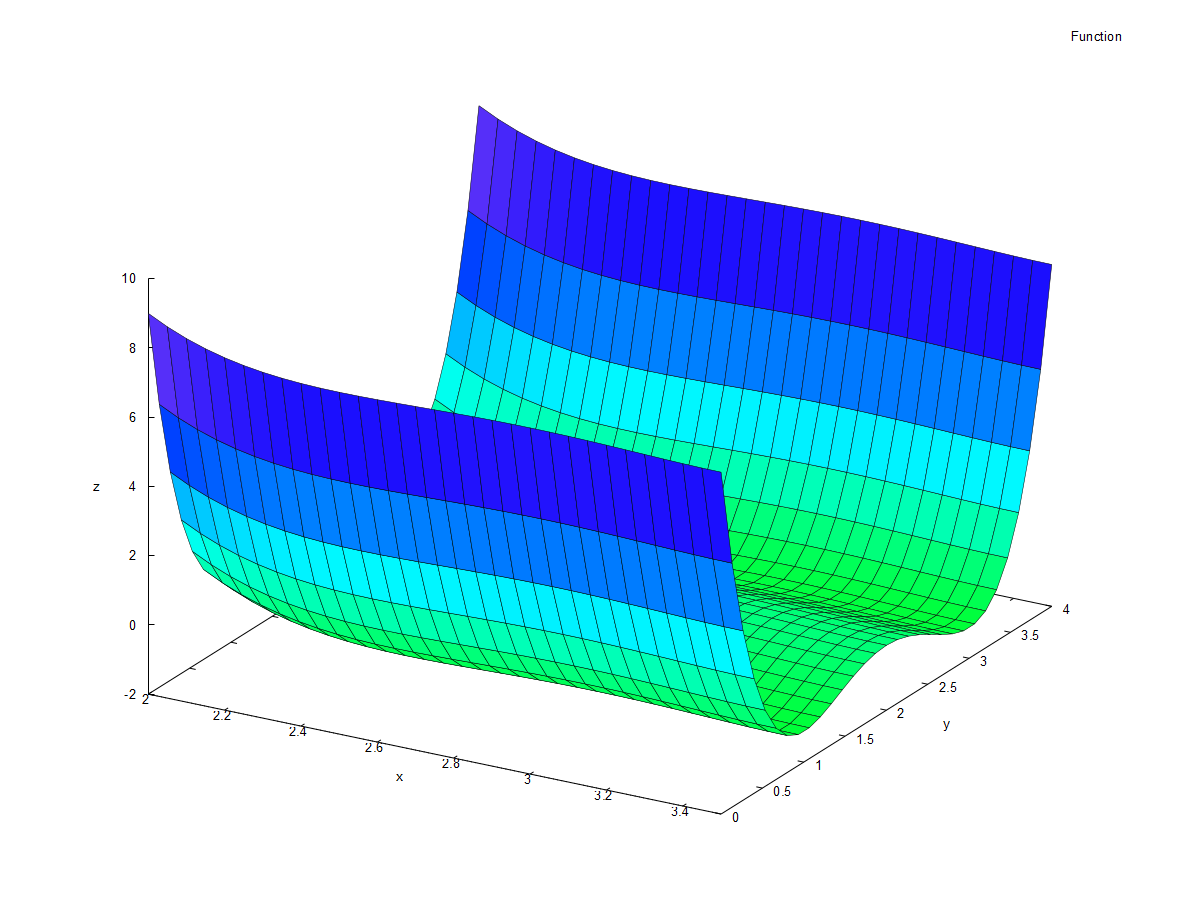
\includegraphics[width=.95\linewidth,height=.80\textheight,keepaspectratio]{maxima_report_img/maxima_report_1}\mbox{}
\]
%%%%%%%%%%%%%%%%


\noindent
%%%%%%%%
%% INPUT:
\begin{minipage}[t]{4.000000em}\color{red}\bfseries
(\% i72)	
\end{minipage}
\begin{minipage}[t]{\textwidth}\color{blue}
wxplot3d(f(x,\ y),\ [x,\ 2,\ 3],\ [y,\ 0.5,1.5])\\
\$
\end{minipage}
%%%% OUTPUT:
\[\displaystyle \tag{\% t72} 
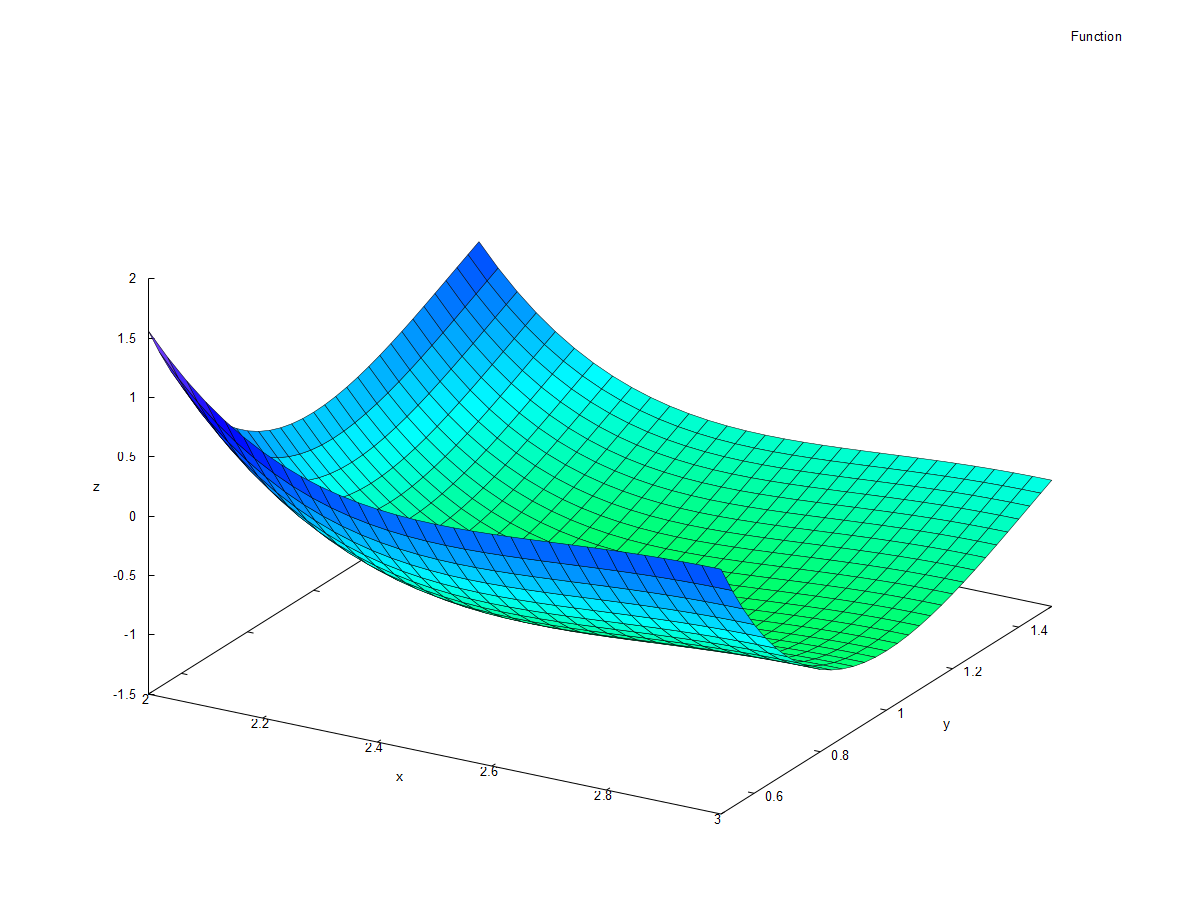
\includegraphics[width=.95\linewidth,height=.80\textheight,keepaspectratio]{maxima_report_img/maxima_report_2}\mbox{}
\]
%%%%%%%%%%%%%%%%


\noindent
%%%%%%%%
%% INPUT:
\begin{minipage}[t]{4.000000em}\color{red}\bfseries
(\% i73)	
\end{minipage}
\begin{minipage}[t]{\textwidth}\color{blue}
wxplot3d(f(x,\ y),\ [x,\ 3,\ 4],\ [y,\ 0.5,1.5])\$
\end{minipage}
%%%% OUTPUT:
\[\displaystyle \tag{\% t73} 
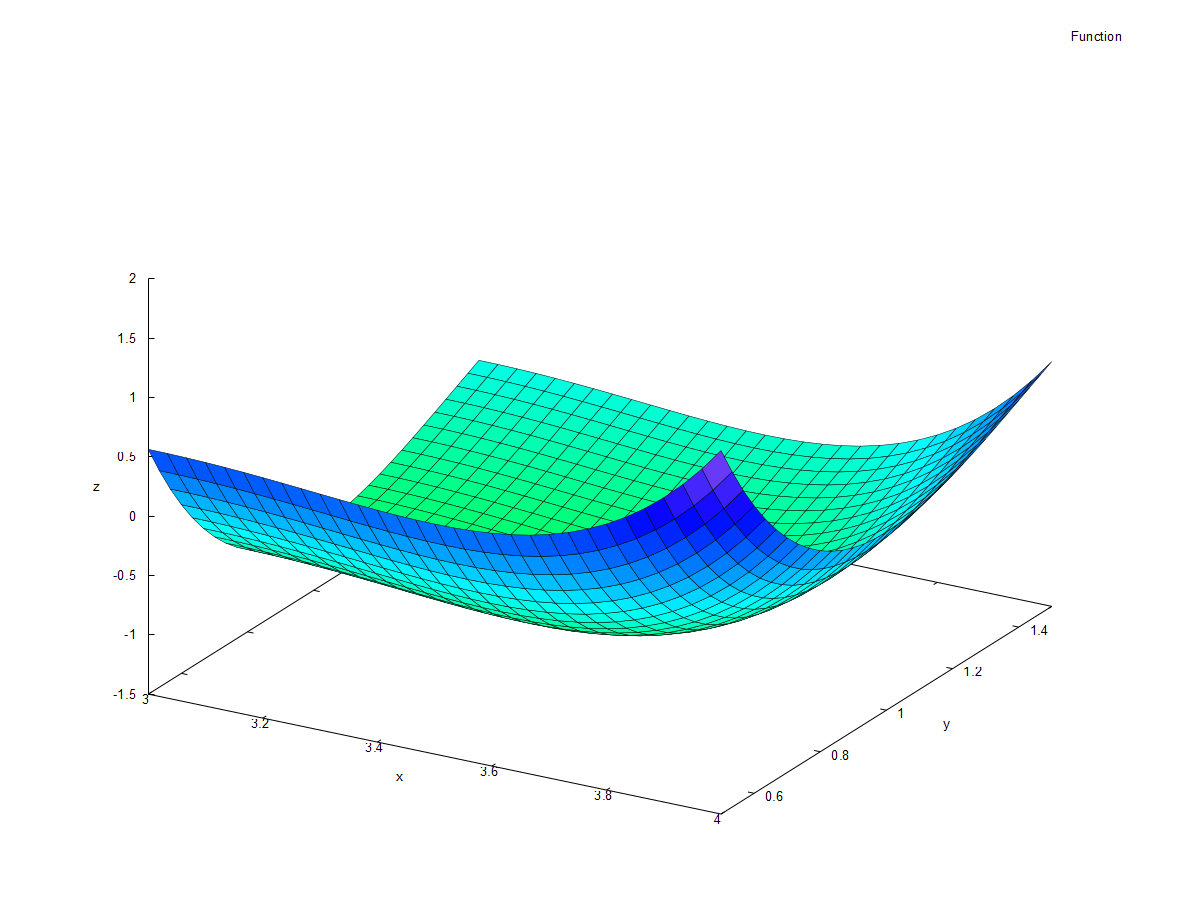
\includegraphics[width=.95\linewidth,height=.80\textheight,keepaspectratio]{maxima_report_img/maxima_report_3}\mbox{}
\]
%%%%%%%%%%%%%%%%


\noindent
%%%%%%%%
%% INPUT:
\begin{minipage}[t]{4.000000em}\color{red}\bfseries
(\% i76)	
\end{minipage}
\begin{minipage}[t]{\textwidth}\color{blue}
wxplot3d(f(x,\ y),\ [x,\ 2.5,\ 3.5],\ [y,\ 1.5,2.5])\$
\end{minipage}
%%%% OUTPUT:
\[\displaystyle \tag{\% t76} 
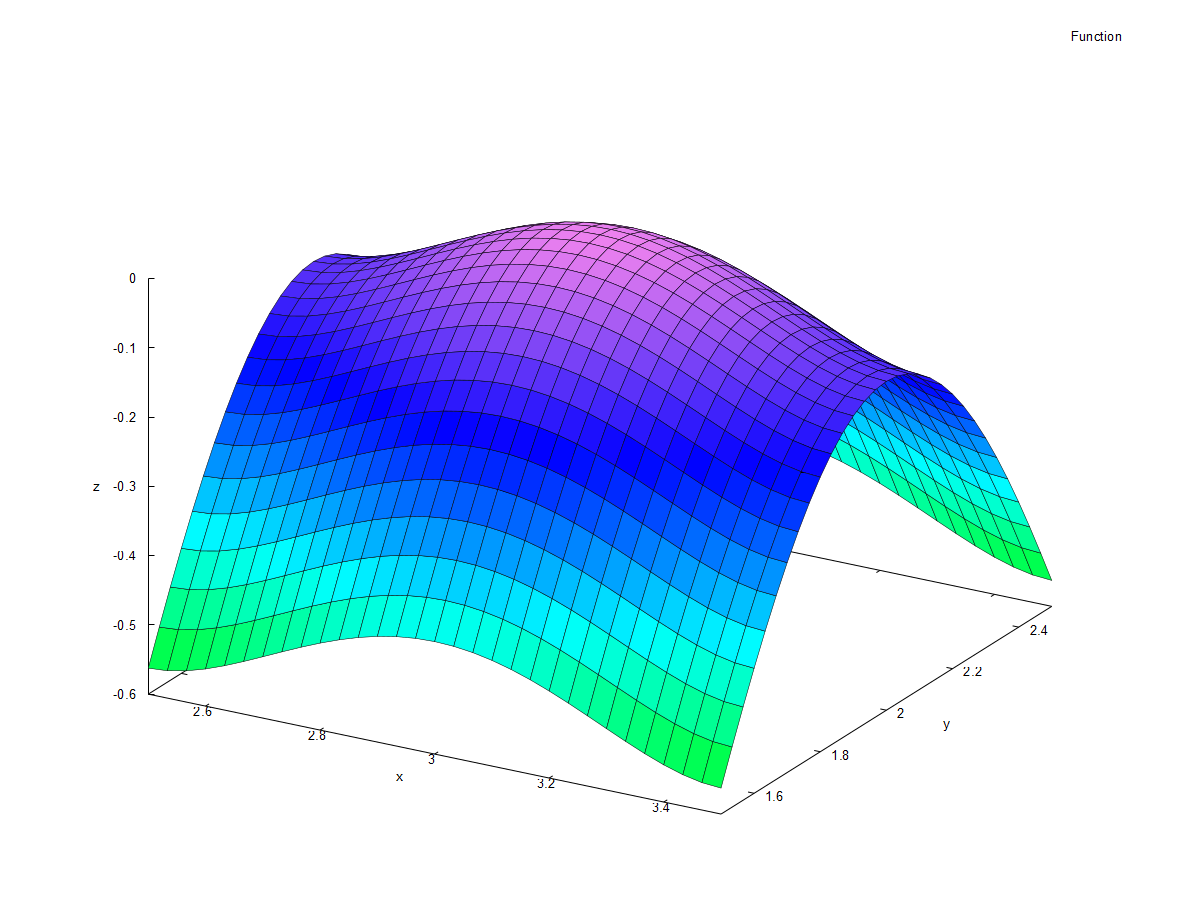
\includegraphics[width=.95\linewidth,height=.80\textheight,keepaspectratio]{maxima_report_img/maxima_report_4}\mbox{}
\]
%%%%%%%%%%%%%%%%


\noindent
%%%%%%%%
%% INPUT:
\begin{minipage}[t]{4.000000em}\color{red}\bfseries
(\% i77)	
\end{minipage}
\begin{minipage}[t]{\textwidth}\color{blue}
wxplot3d(f(x,\ y),\ [x,\ 2,\ 3],\ [y,\ 2.5,3.5]);
\end{minipage}
%%%% OUTPUT:
\[\displaystyle \tag{\% t77} 
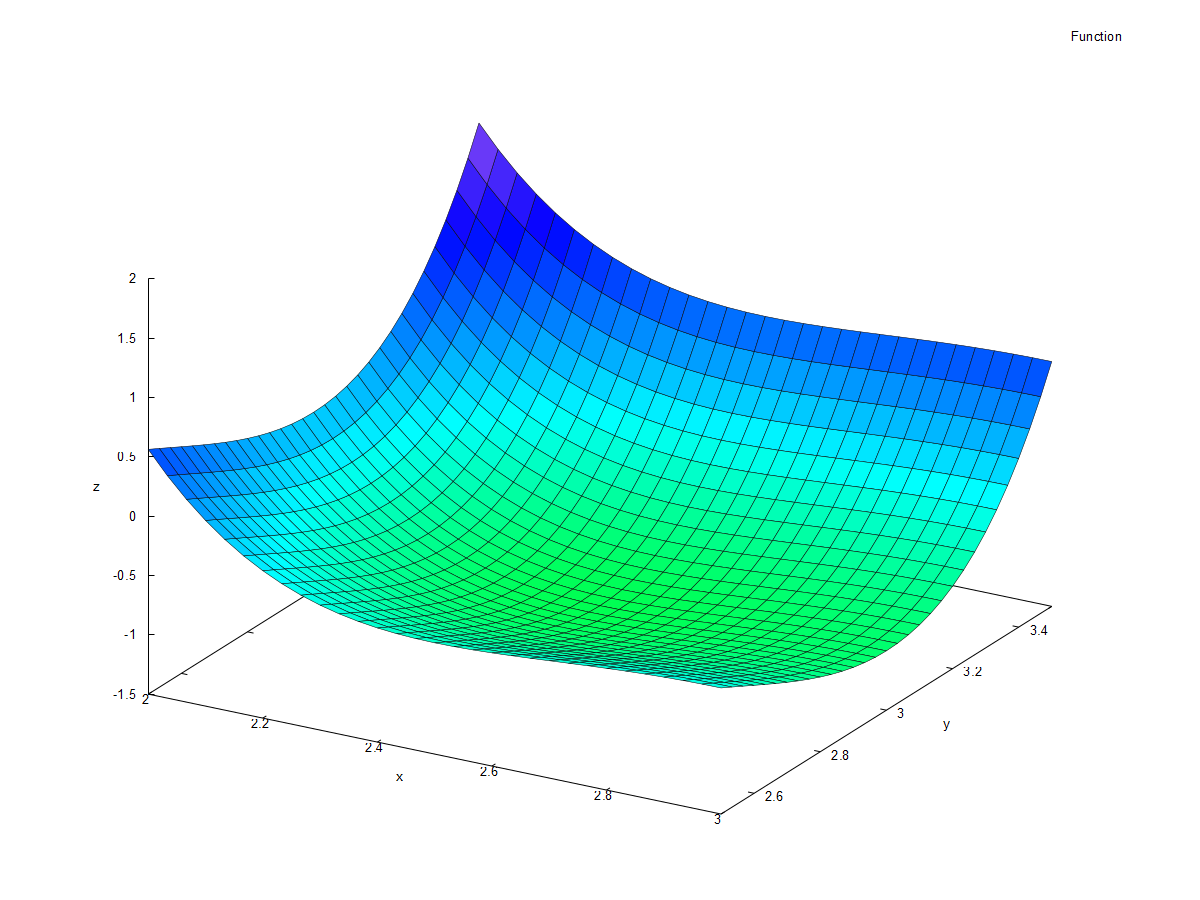
\includegraphics[width=.95\linewidth,height=.80\textheight,keepaspectratio]{maxima_report_img/maxima_report_5}\mbox{}\]

\[\tag{\% o77} 
\mbox{}
\]
%%%%%%%%%%%%%%%%


\noindent
%%%%%%%%
%% INPUT:
\begin{minipage}[t]{4.000000em}\color{red}\bfseries
(\% i80)	
\end{minipage}
\begin{minipage}[t]{\textwidth}\color{blue}
wxplot3d(f(x,\ y),\ [x,\ 3,\ 4],\ [y,\ 2.5,3.5]);
\end{minipage}
%%%% OUTPUT:
\[\displaystyle \tag{\% t80} 
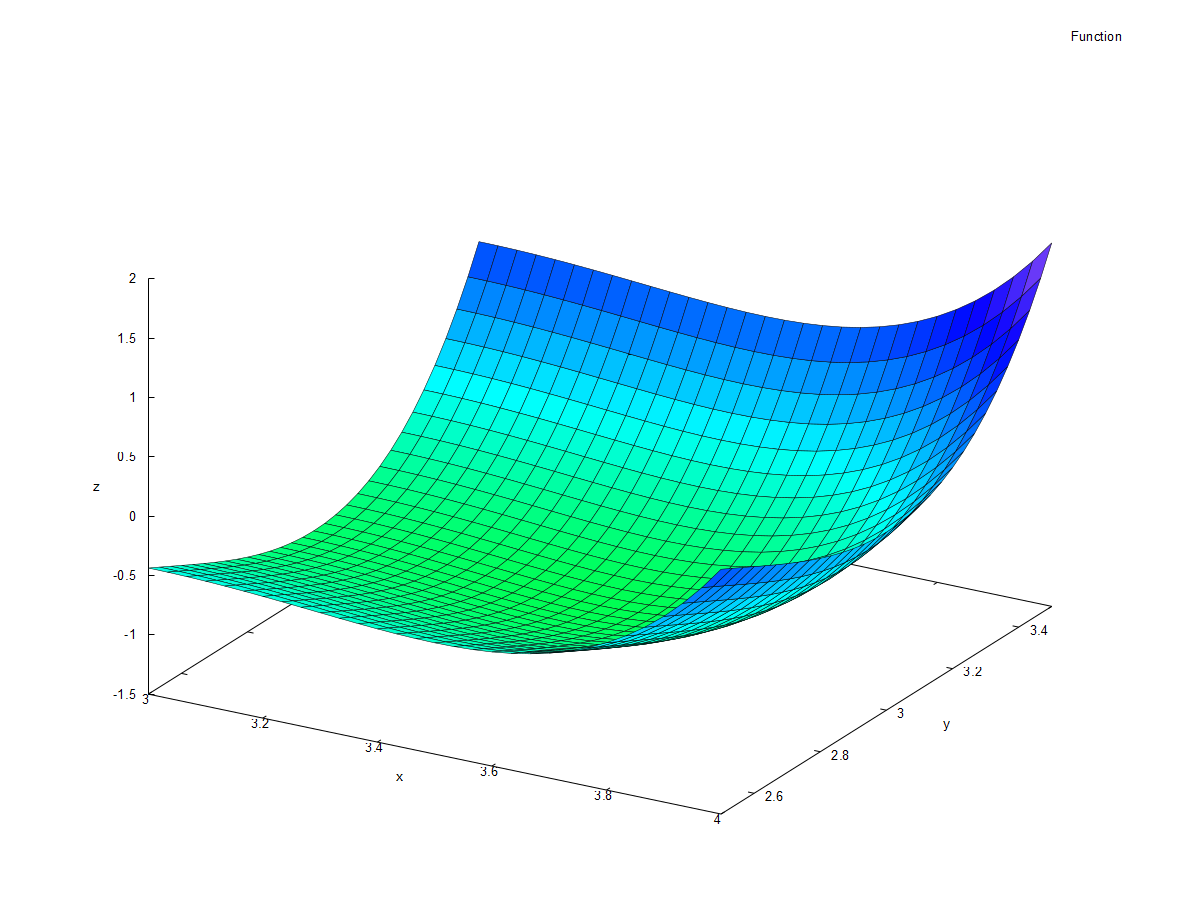
\includegraphics[width=.95\linewidth,height=.80\textheight,keepaspectratio]{maxima_report_img/maxima_report_6}\mbox{}\]

\[\tag{\% o80} 
\mbox{}
\]
%%%%%%%%%%%%%%%%

\section{Заключение}
\begin{itemize}
    \item Была поставлена цель по исследованию функции двух переменных на экстремум. 
    \item В ходе работы была использована система компьютерной алгебры Maxima и Gnuplot для построения графиков.
    \item Из 9 полученных точек 5 оказались точками экстремума - одна на максимум и 4 на минимум.
\end{itemize}

\end{document}
